% Options for packages loaded elsewhere
\PassOptionsToPackage{unicode}{hyperref}
\PassOptionsToPackage{hyphens}{url}
%
\documentclass[
]{article}
\usepackage{amsmath,amssymb}
\usepackage{lmodern}
\usepackage{iftex}
\ifPDFTeX
  \usepackage[T1]{fontenc}
  \usepackage[utf8]{inputenc}
  \usepackage{textcomp} % provide euro and other symbols
\else % if luatex or xetex
  \usepackage{unicode-math}
  \defaultfontfeatures{Scale=MatchLowercase}
  \defaultfontfeatures[\rmfamily]{Ligatures=TeX,Scale=1}
\fi
% Use upquote if available, for straight quotes in verbatim environments
\IfFileExists{upquote.sty}{\usepackage{upquote}}{}
\IfFileExists{microtype.sty}{% use microtype if available
  \usepackage[]{microtype}
  \UseMicrotypeSet[protrusion]{basicmath} % disable protrusion for tt fonts
}{}
\makeatletter
\@ifundefined{KOMAClassName}{% if non-KOMA class
  \IfFileExists{parskip.sty}{%
    \usepackage{parskip}
  }{% else
    \setlength{\parindent}{0pt}
    \setlength{\parskip}{6pt plus 2pt minus 1pt}}
}{% if KOMA class
  \KOMAoptions{parskip=half}}
\makeatother
\usepackage{xcolor}
\usepackage[margin=1in]{geometry}
\usepackage{graphicx}
\makeatletter
\def\maxwidth{\ifdim\Gin@nat@width>\linewidth\linewidth\else\Gin@nat@width\fi}
\def\maxheight{\ifdim\Gin@nat@height>\textheight\textheight\else\Gin@nat@height\fi}
\makeatother
% Scale images if necessary, so that they will not overflow the page
% margins by default, and it is still possible to overwrite the defaults
% using explicit options in \includegraphics[width, height, ...]{}
\setkeys{Gin}{width=\maxwidth,height=\maxheight,keepaspectratio}
% Set default figure placement to htbp
\makeatletter
\def\fps@figure{htbp}
\makeatother
\setlength{\emergencystretch}{3em} % prevent overfull lines
\providecommand{\tightlist}{%
  \setlength{\itemsep}{0pt}\setlength{\parskip}{0pt}}
\setcounter{secnumdepth}{-\maxdimen} % remove section numbering
\newlength{\cslhangindent}
\setlength{\cslhangindent}{1.5em}
\newlength{\csllabelwidth}
\setlength{\csllabelwidth}{3em}
\newlength{\cslentryspacingunit} % times entry-spacing
\setlength{\cslentryspacingunit}{\parskip}
\newenvironment{CSLReferences}[2] % #1 hanging-ident, #2 entry spacing
 {% don't indent paragraphs
  \setlength{\parindent}{0pt}
  % turn on hanging indent if param 1 is 1
  \ifodd #1
  \let\oldpar\par
  \def\par{\hangindent=\cslhangindent\oldpar}
  \fi
  % set entry spacing
  \setlength{\parskip}{#2\cslentryspacingunit}
 }%
 {}
\usepackage{calc}
\newcommand{\CSLBlock}[1]{#1\hfill\break}
\newcommand{\CSLLeftMargin}[1]{\parbox[t]{\csllabelwidth}{#1}}
\newcommand{\CSLRightInline}[1]{\parbox[t]{\linewidth - \csllabelwidth}{#1}\break}
\newcommand{\CSLIndent}[1]{\hspace{\cslhangindent}#1}
\usepackage{longtable}
\usepackage{geometry}
\usepackage{lscape}
\usepackage{caption}
\usepackage{tikz}
\usepackage{graphicx}
\usepackage{fullpage}
\usepackage{anysize}
\usepackage{pdflscape}
\ifLuaTeX
  \usepackage{selnolig}  % disable illegal ligatures
\fi
\IfFileExists{bookmark.sty}{\usepackage{bookmark}}{\usepackage{hyperref}}
\IfFileExists{xurl.sty}{\usepackage{xurl}}{} % add URL line breaks if available
\urlstyle{same} % disable monospaced font for URLs
\hypersetup{
  hidelinks,
  pdfcreator={LaTeX via pandoc}}

\author{}
\date{\vspace{-2.5em}}

\begin{document}

\newcommand*{\BaseDir}{P:/OFPSAM/Cty_status_reports/ISNRs/Country_TFAR/2023/Report_template}
\newcommand*{\FigDir}{P:/OFPSAM/TFAR/T_FAR_2022/figs/}

\AddToHook{shipout/firstpage}{%
    \put (-1in,-10.5in){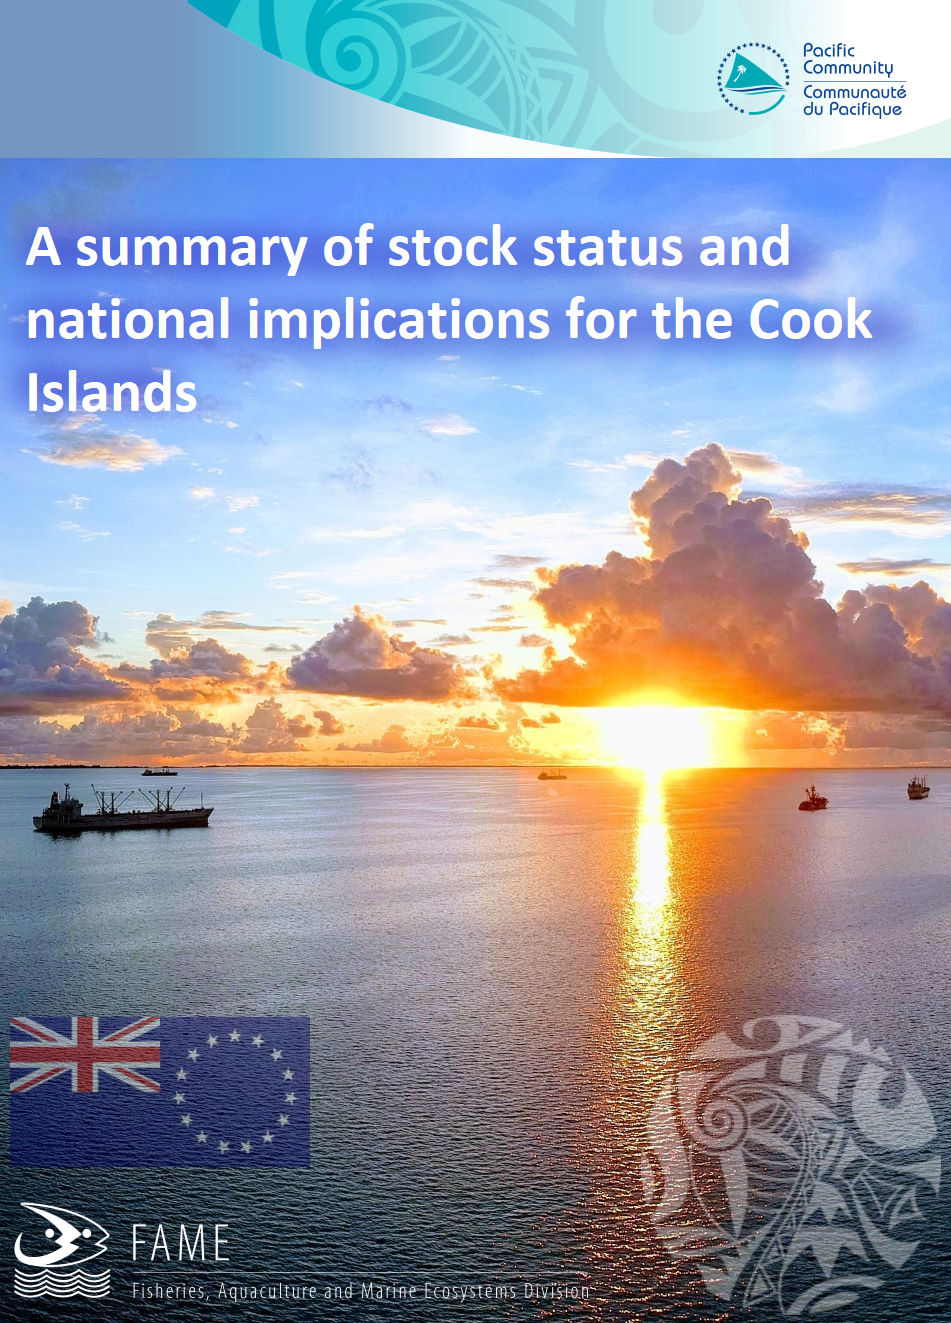
\includegraphics[width=\paperwidth,height=\paperheight]{P:/OFPSAM/Cty_status_reports/ISNRs/Country_TFAR/2023/Report_template/Graphics/CT_TFAR_Title_Template_CTexple.jpg}}%
}

\hspace{1cm}

\newpage

\hypertarget{executive-summary}{%
\section{Executive summary}\label{executive-summary}}

Text

\clearpage

\hypertarget{introduction}{%
\section{Introduction}\label{introduction}}

Tuna stock assessments provide important information regarding the
status of regional tuna stocks and the future predicted impacts of
fishing on them. This information can help the Solomon Islands and other
WCPFC members decide how best to collectively manage these stocks.

Albacore, bigeye, yellowfin and skipjack tuna are targeted by fisheries
operating in the Solomon Islands. The SPC has assessed these stocks in
the WCPFC-CA using a modeling tool called MULTIFAN-CL, which is reliant
on accurate and comprehensive catch, effort, size and other fisheries
data collected by all fishing nations. The assessments provide
information on stock status at the WCPFC-CA scale and broad model
Regions within that. SPC is working to develop models that can provide
similar information at the EEZ scale. However, given that tuna are
migratory and may pass through many EEZ's in their lifetime, it will
never be feasible to assess and/or manage these species within
individual EEZ's in isolation from what is happening in surrounding
waters. However, most countries also need to know what the status of the
resource is in their immediate vicinity. Therefore we provide here some
information for the broad model region that surrounds your EEZ so that
you can assess your country's impact on the stock and the state of the
stock in your waters.

This report should be used in conjunction with the Tuna Fisheries
Assessment Report published annually by the SPC (Brouwer et al. 2019).
Tuna stock assessment results are described using a number of technical
terms, and refer to a number of key indicators of stock status
(reference points). These terms are described in \autoref{tab1}.

\begingroup\fontsize{9pt}{11pt}\selectfont
\begin{longtable}{p{5cm}p{10cm}}
\caption{Definitions of key terms used in describing the impact of fishing upon and the status of fish stocks} \\ 
  \hline
\hline
Term & Definition \\ 
  \hline
Depletion & Depletion describes the level of reduction in the fish stock since fishing first began, typically by comparing current spawning biomass to that which would occur if there was no fishing (SB$_{current}$/SB$_{F=0}$). \\ \\
   Fishing mortality rate & The proportion of the stock removed by fishing in a unit of time. \\ \\
  Growth overfished & Fish are harvested at an average size that is smaller than the size that would produce the maximum yield per recruit. \\ \\
   Maximum Sustainable Yield (MSY) & The maximum amount of catch that can be taken from the stock per year, on average, in the long-term \\ \\
  Overfished fishery  & Occurs when there are no longer enough adults in the population to produce enough young to replace those fish removed from the population by fishing.  In the WCPFC, an overfished fishery is defined as one where the current spawning biomass (SB$_{current}$) is less than 20\% of the spawning biomass in the absence of fishing (SB$_{F=0}$).  \\ \\
   Overfishing  & In the WCPFC, overfishing is defined as occurring when the current fishing mortality rate exceeds the fishing mortality rate that would provide the maximum sustainable yield. Sustained overfishing leads to an overfished state. \\ \\
  Recruitment overfished & Occurs when the adult population is depleted to a level where it no longer has the reproductive capacity to replenish itself. \\ \\
   \hline
\hline
\label{tab1}
\end{longtable}
\endgroup


\hypertarget{summary-of-tuna-stock-status}{%
\section{Summary of tuna stock
status}\label{summary-of-tuna-stock-status}}

The most recent assessments indicate that overfishing is not occurring
on albacore, bigeye, skipjack and yellowfin tuna, and these stocks are
not in an overfished state (\autoref{fig1}). However, catch of each of
these species have increased significantly over the past 2 to 3 decades,
with corresponding reductions in stock biomass relative to the biomass
that would be in the water if no fishing was occurring. The following
sections provide more detail regarding the status of these stocks,
implications for your national fisheries and briefly reviews assessments
of other relevant species. Specific details regarding catch and stock
status of each species in the WCPFC and your EEZ are presented in
\autoref{tab2}.

\begin{figure}[!ht]
  \centering
 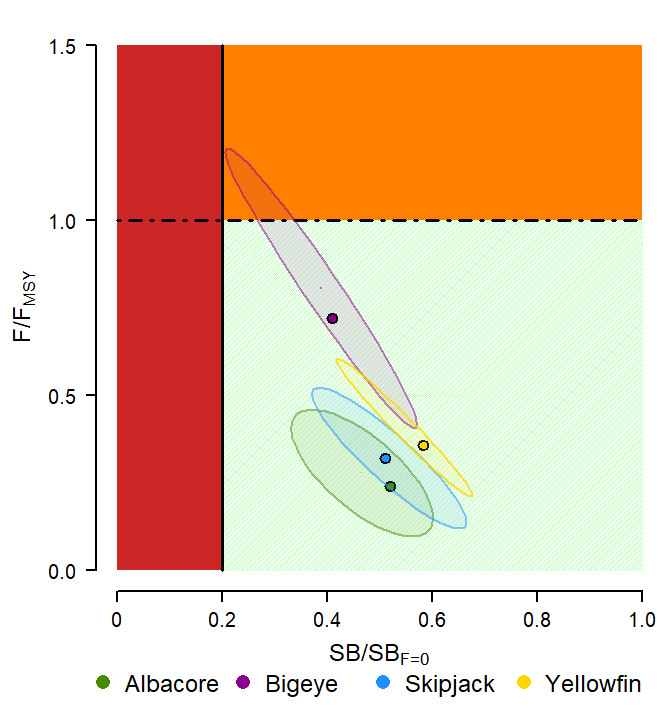
\includegraphics [width=13cm]{Fig16-majuro.ellipses.png} 
  \caption {Majuro plot comparing the stock status of the key target tuna species caught in the WCPFC Convention Area. Where current fishing mortality rate exceeds the fishing mortality rate at MSY (F/F$_{MSY}$ > 1) then overfishing is occurring. Where the current spawning biomass is less than 0.2 of spawning biomass without fishing, then the stock is overfished (SB/SB$_{F=0}$ <0.2). The large points represent the median estimated stock status in terms of fishing mortality and biomass depletion in the terminal year of the most recent assessment for each species. The error bars indicate stock status uncertainty from all models run in the grid. The blue and green dashed lines indicate the WCPFC interim target reference points for skipjack and albacore tuna, respectively.\label{fig1}}  
\end{figure}

% latex table generated in R 3.6.1 by xtable 1.8-4 package
% Fri Dec 11 16:20:55 2020
\begingroup\fontsize{8pt}{11pt}\selectfont
\begin{longtable}{lcccc}
\caption{Key fishery statistics averaged from 2014 to 2019 for each of the four main target tunas.} \\ 
  \hline
\hline
{\small{{Recent Average Catch (2014 - 2019)}}} & {\small{{Skipjack}}} & {\small{{Yellowfin}}} & {\small{{Bigeye}}} & {\small{{SP Albacore}}} \\ 
  \hline
WCPFC-CA catch & 1,811,054 & 682,741 & 142,668 & 67,486 \\ 
  5 year WCPFC-CA catch trend & Increasing & Increasing & Decreasing & Increasing \\ 
  WCPFC-CA Longline catch & 4,277 & 98,076 & 67,831 & 64,437 \\ 
  WCPFC-CA Purse seine catch & 1,432,585 & 397,691 & 56,537 & 8 \\ 
  WCPFC-CA Pole and line catch & 153,614 & 25,613 & 3,493 & 26 \\ 
  WCPFC-CA Other catch & 220,579 & 161,362 & 14,807 & 3,016 \\ 
  Fishing impacts &  &  &  &  \\ 
   Percent reduction in spawning biomass in region & 47 & 72 & 44 & 48 \\ 
  Percent reduction in spawning biomass in WCPFC-CA & 48 & 59 & 56 & 42 \\ 
  Local implications &  &  &  &  \\ 
   Catch in model Region & 659,894 & 126,291 & 50,521 & 34,719 \\ 
  Percent WCPFC catch from model Region & 36.4 & 18.5 & 35.4 & 51.4 \\ 
  Recent average catch in CK (2015 - 2019) & 18,514 & 2,896 & 1,147 & 4,396 \\ 
  Percent WCPFC-CA catch in CK & 1 & 0.4 & 0.8 & 6.5 \\ 
  Recent average catch by CK outside EEZ & 377 & 203 & 127 & 498 \\ 
  Percent WCPFC-CA catch by CK outside your EEZ & <0.1 & <0.1 & <0.1 & 0.7 \\ 
   \hline
\hline
\label{tab2}
\end{longtable}
\endgroup


\hypertarget{skipjack-tuna}{%
\section{Skipjack tuna}\label{skipjack-tuna}}

The most recent skipjack tuna assessment was conducted in 2019 (Vincent,
Pilling, and Hampton 2019). The skipjack assessment used an eight region
model, which was a change from the five region model previously used in
previous assessment; your EEZ is situated in \textbf{skjreg}
(\autoref{fig2} - top). Between \textbf{minyear} and \textbf{maxyear}
skipjack catch averaged \textbf{tabl2}t in the WCPFC-CA (\autoref{fig2}
- middle). An average of \textbf{tabl2}t (\textbf{tabl2}\% of WCPFC-CA
catch) comes from \textbf{skjreg}. It is estimated that skipjack
spawning biomass in the WCPFC-CA and \textbf{skjreg}, have been reduced
through fishing by \textbf{tabl2}\% and \textbf{tabl2}\% respectively
(\autoref{tab2}). The greatest impacts on spawning biomass in the WCPO
are equally from the FAD-associated and free school purse seine
fisheries, while the FAD-associated purse seine fishery has the greatest
impact in \textbf{skjreg} (\autoref{fig2} - bottom).

The SC15 of the WCPFC concluded that overfishing is not occurring on the
skipjack stock and the stock is not overfished (\autoref{fig1}). The
spawning biomass level is below the interim Target Reference Point of
50\% (\(SB/SB_{F=0}\) = 0.5), though well above the Limit Reference
Point of 20\%, unfished spawning biomass. Previously, the SC12 noted
that fishing is having a significant impact on stock size, especially in
the western equatorial region and can be expected to negatively affect
catch rates. The stock distribution is also influenced by changes in
oceanographic conditions associated with El Ni\textasciitilde\{n\}o and
La Ni\textasciitilde\{n\}a events, which impact on catch rates and stock
size. Additional purse-seine effort will yield only modest gains in
long-term skipjack catch and may result in a corresponding increase in
fishing mortality for bigeye and yellowfin tunas \textbf{WCPFC2019}.

Annual catch of skipjack in the Solomon Islands has averaged
\textbf{tabl2}t between \textbf{minyear} and \textbf{maxyear},
representing \textbf{tabl2}\% of WCPFC-CA and \textbf{tabl2}\% of
\textbf{skjreg} skipjack catch. Together, skipjack catch inside the
Solomon Islands and by the Solomon Islands fleet outside your EEZ have
accounted for an average \textbf{tabl2}\% of the WCPFC skipjack catch.
Regional catch of skipjack tuna, including those within or by the
Solomon Islands, are considered sustainable at recent average levels.
However, the Solomon Islands should note that the FAD component of the
regional purse seine fishery (the main fishery for skipjack tuna)
catches juvenile bigeye and yellowfin tuna, and that fishery is
contributing to the impact on these stocks.

\clearpage

\begin{figure}[!ht]
 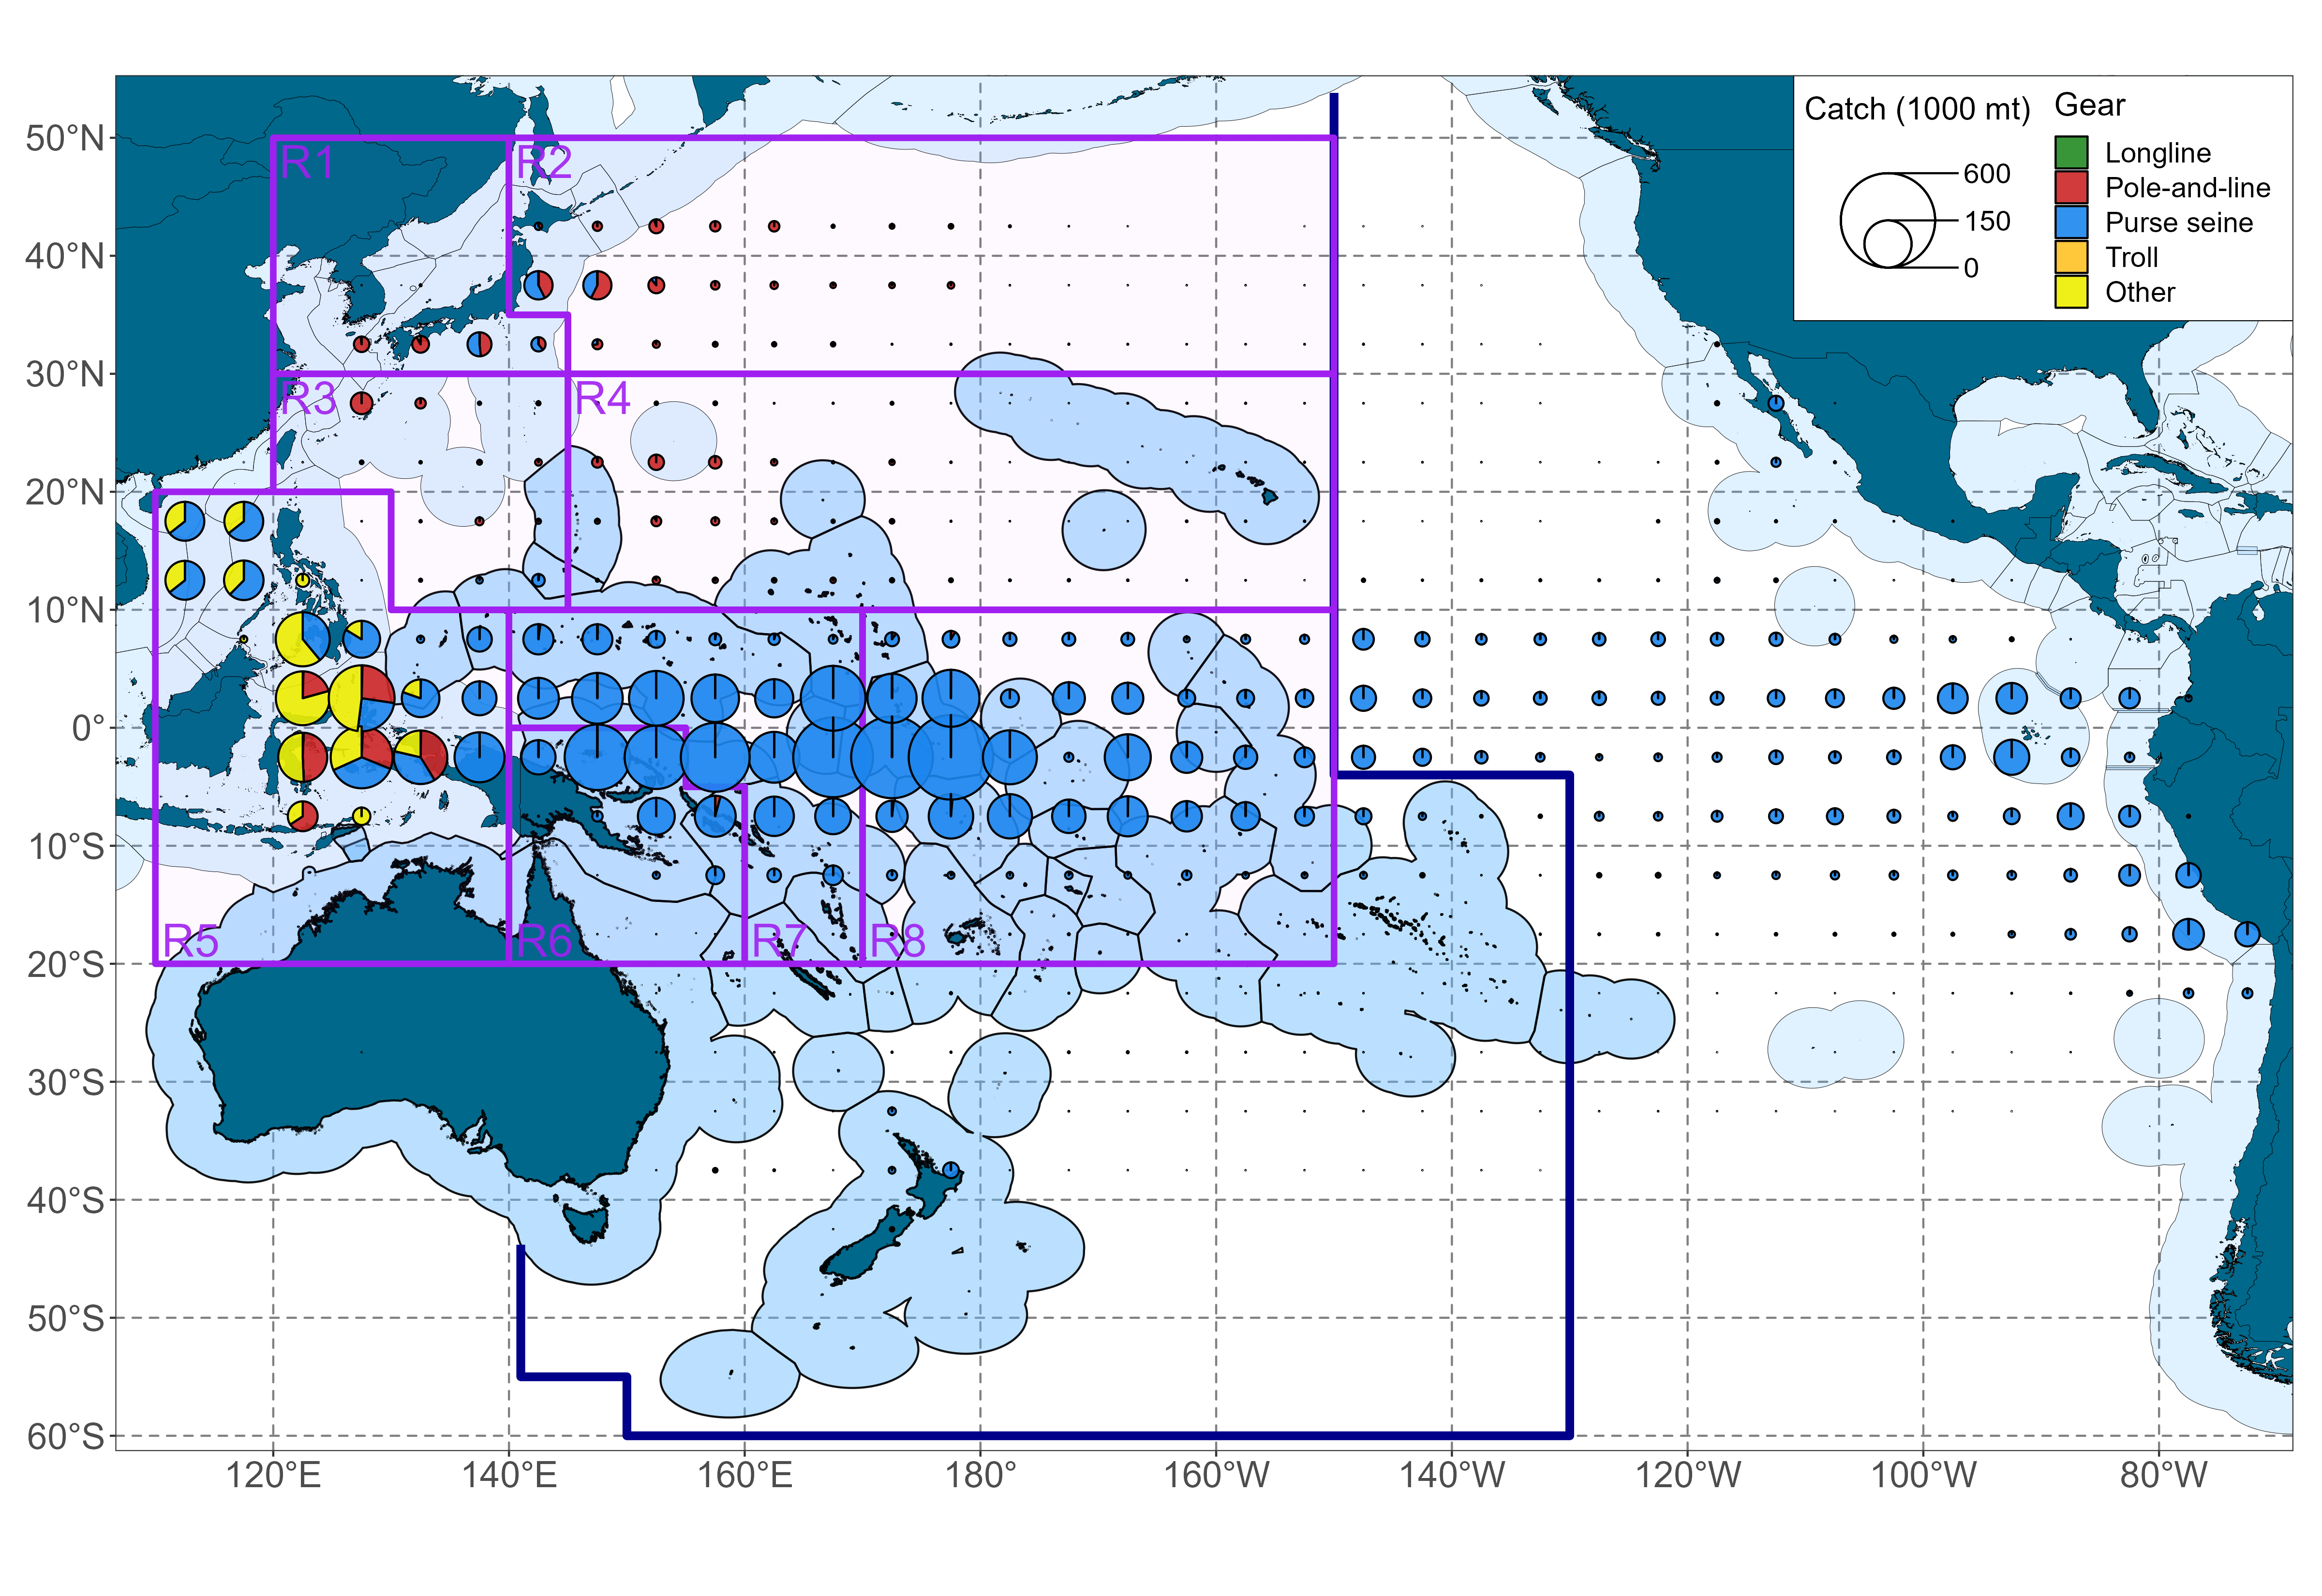
\includegraphics [width=15.5cm]{Fig08b-skj_mapE.png}
 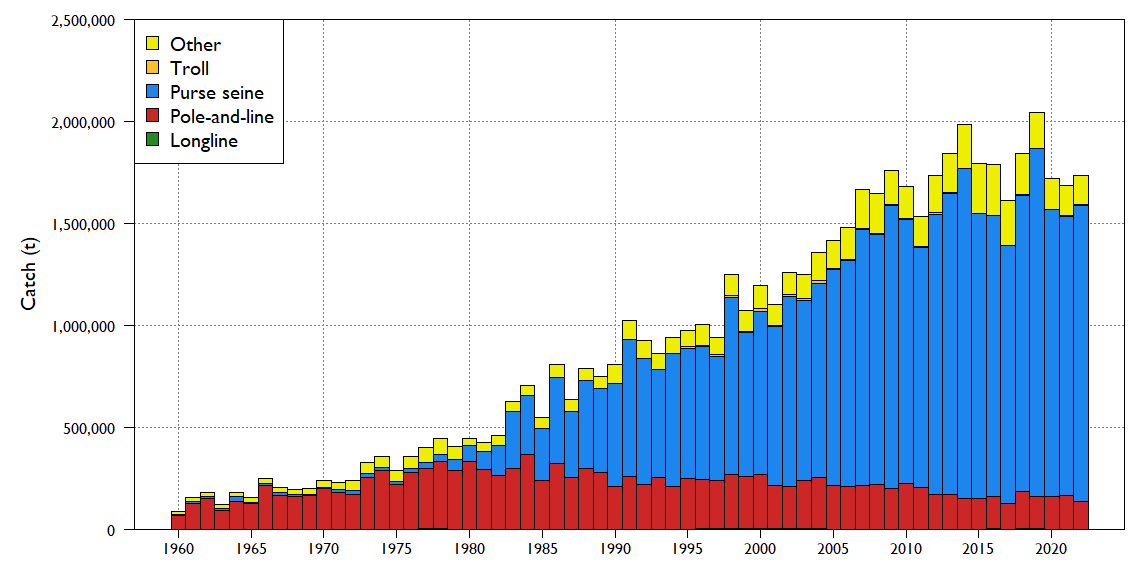
\includegraphics [width=15cm]{Fig08a-skj_catchbygearE.png}
  \caption {Distribution of total .\label{fig2}}
\end{figure}
\clearpage

\hypertarget{yellowfin-tuna}{%
\section{Yellowfin tuna}\label{yellowfin-tuna}}

The most recent yellowfin tuna assessment was conducted in 2017
\textbf{TremblayBoyer2017}. The yellowfin tuna assessment used a nine
region model, with the Solomon Islands situated in \textbf{yftreg}
(\autoref{fig3} - top). Between \textbf{minyear} and \textbf{maxyear}
yellowfin catch averaged \textbf{tabl2}t in the WCPFC-CA (\autoref{fig3}
- middle). An average of \textbf{tabl2}t (\textbf{tabl2}\% of WCPFC-CA
catch) comes from \textbf{yftreg}. It is estimated that yellowfin
spawning biomass in the WCPFC-CA and \textbf{yftreg}, have declined by
\textbf{tabl2}\% and \textbf{tabl2}\% respectively (\autoref{tab2}). The
greatest impact on the stock is from the fisheries of the Philippines
and Indonesia, along with the FAD directed purse-seine fishery in the
WCPO and from the FAD directed purse-seine fishery in \textbf{yftreg}
(\autoref{fig3} - bottom).

The \textbf{SC13} concluded that overfishing is not occurring on the
yellowfin stock and the stock is not overfished (\autoref{fig1}).
However, fishing mortality, exploitation rates and depletion differ
between regions, and exploitation rates are highest in the equatorial
region (Regions 3, 4, 7 and 8), which account for 94\% of the total
yellowfin tuna catch. The \textbf{SC13} recommended that there be no
increase in yellowfin catch and that measures be implemented to maintain
current spawning biomass levels \textbf{WCPFC2017}.

Annual catch of yellowfin in the Solomon Islands have averaged
\textbf{tabl2}t between \textbf{minyear} and \textbf{maxyear},
representing \textbf{tabl2}\% of WCPFC-CA and \textbf{tabl2}\% of
\textbf{yftreg} yellowfin catch. Together, yellowfin catch inside the
Solomon Islands and by the Solomon Islands fleet outside your EEZ have
accounted for an average \textbf{tabl2}\% of the WCPFC yellowfin catch.
As such, the the Solomon Islands fishery does not contribute
significantly to overall regional impacts on the stock. The yellowfin
stock in \textbf{yftreg} has low levels of depletion in Region 6 but
higher in Region 4 and overall the Solomon Islands catch is a small
percentage of the catch in these two regions.

\clearpage

\begin{figure}[!ht]
 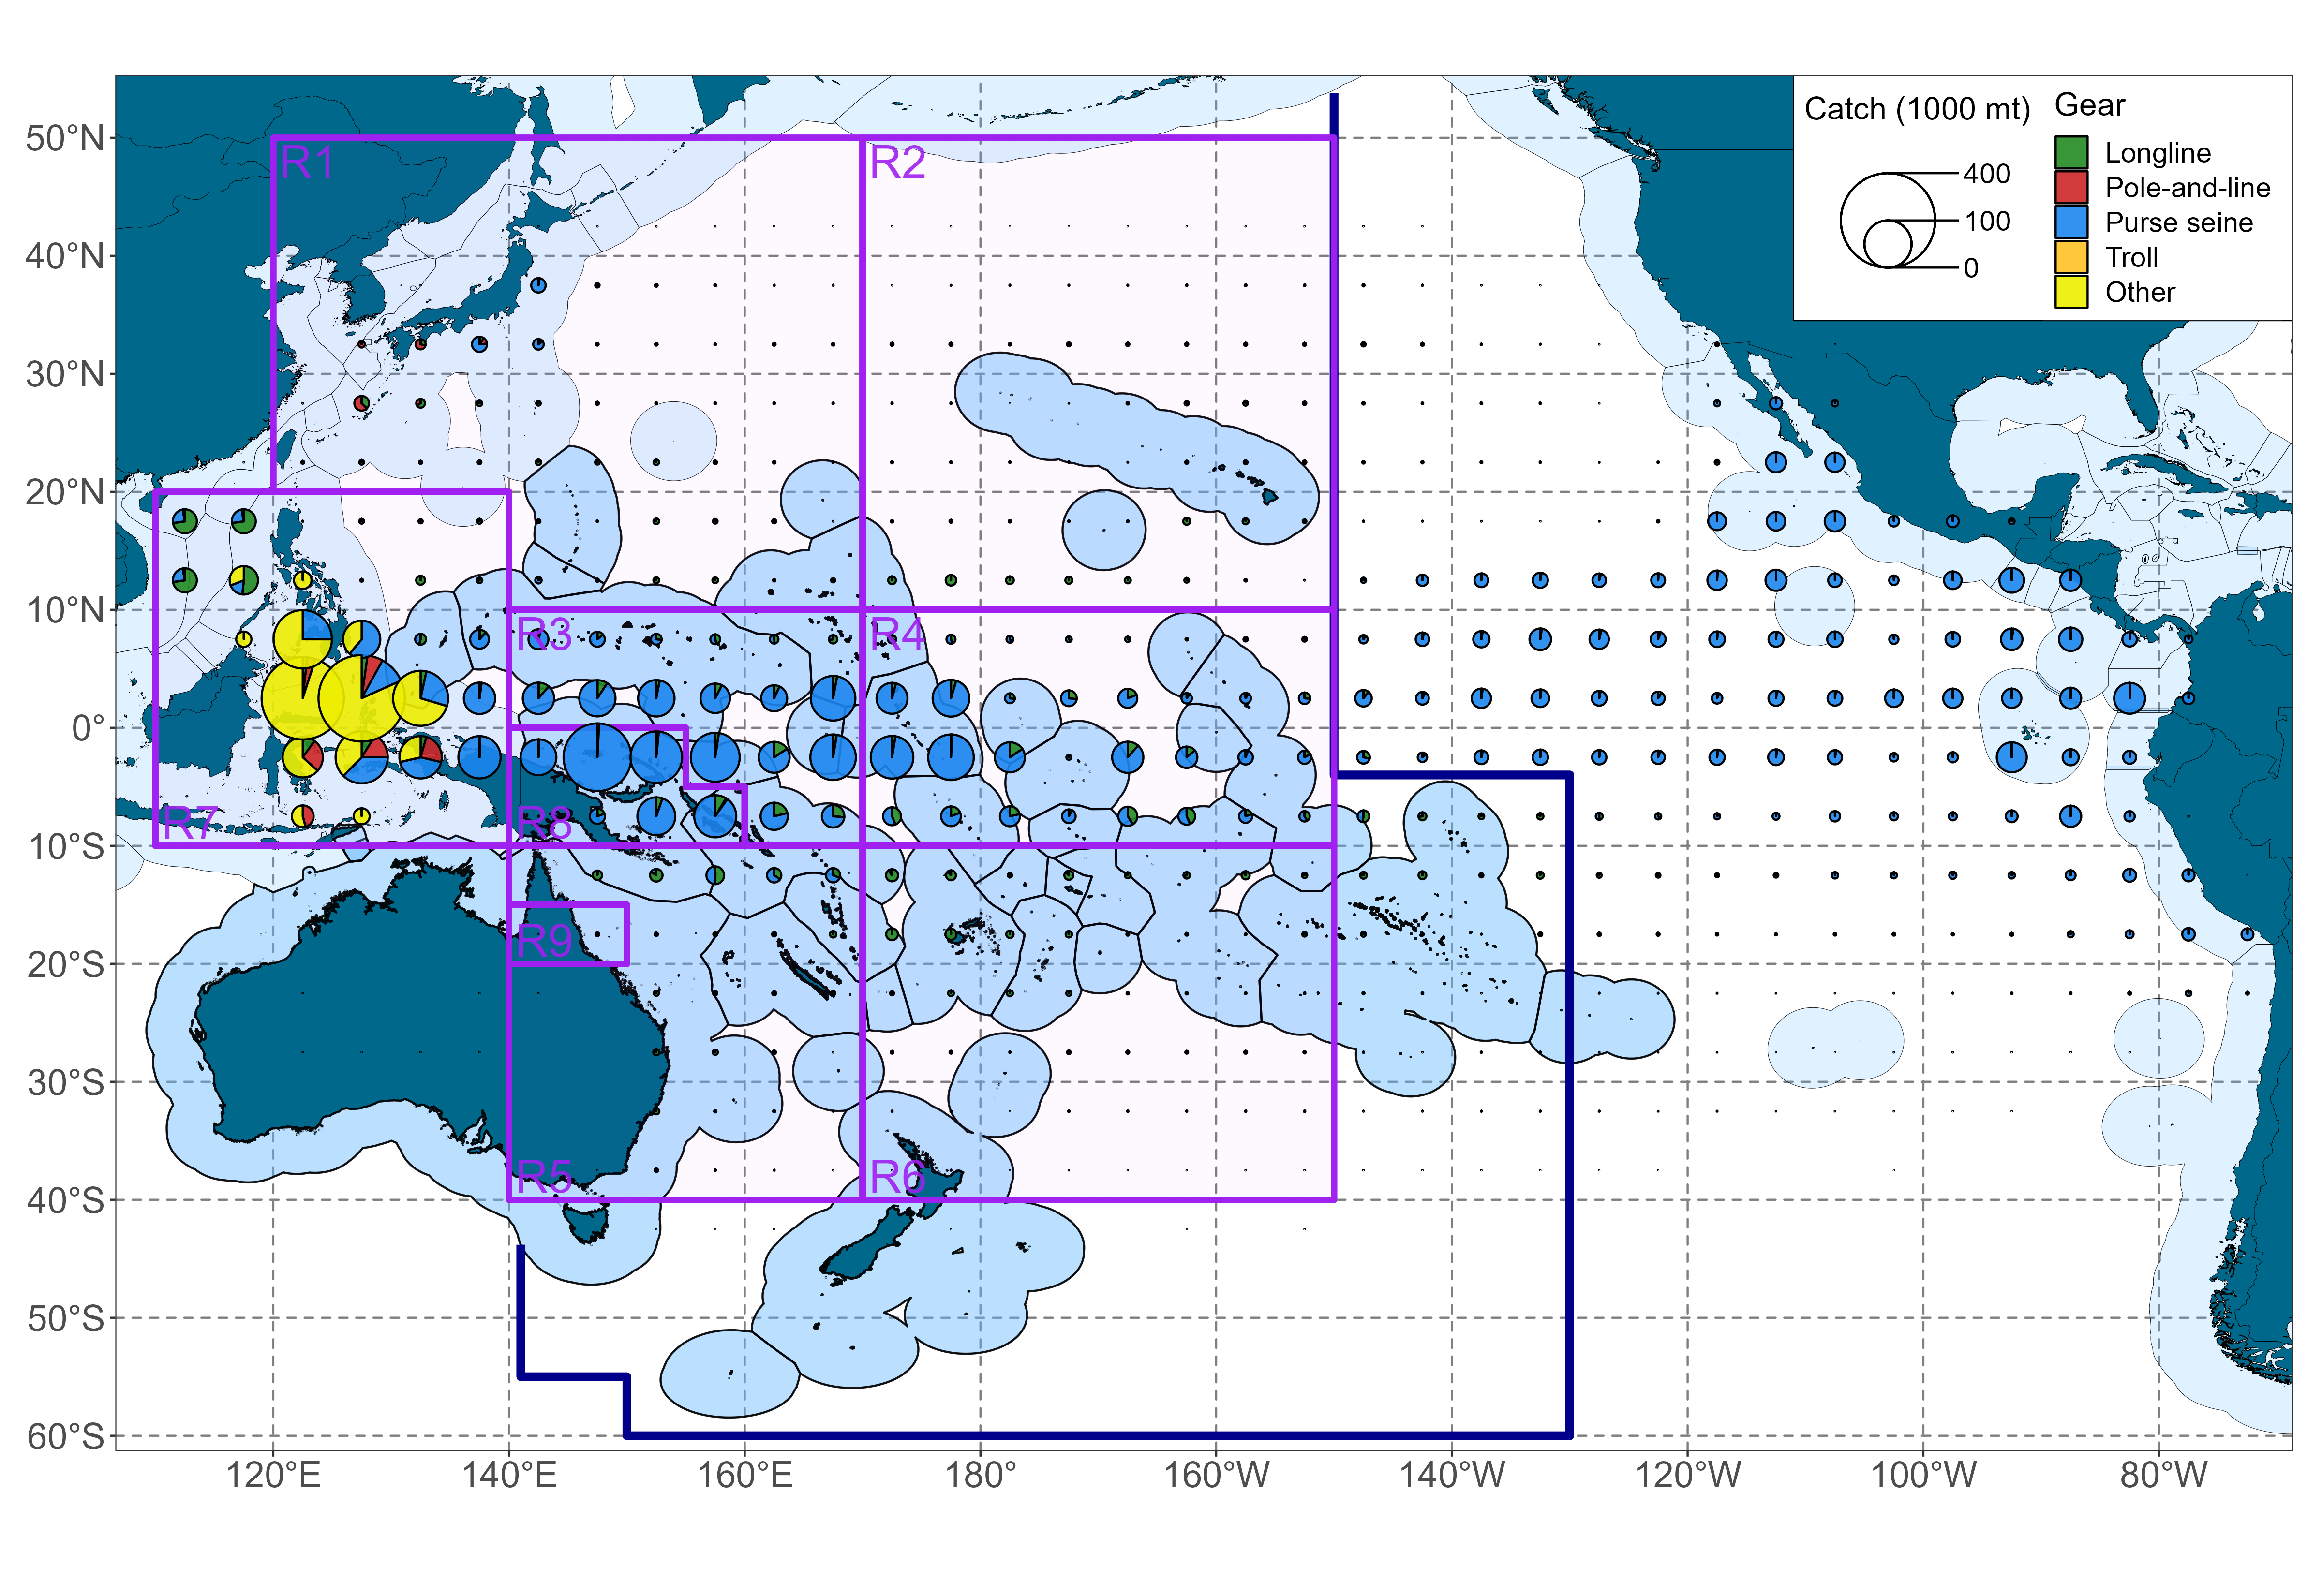
\includegraphics [width=15.5cm]{Fig10b-yft_mapE.png}
 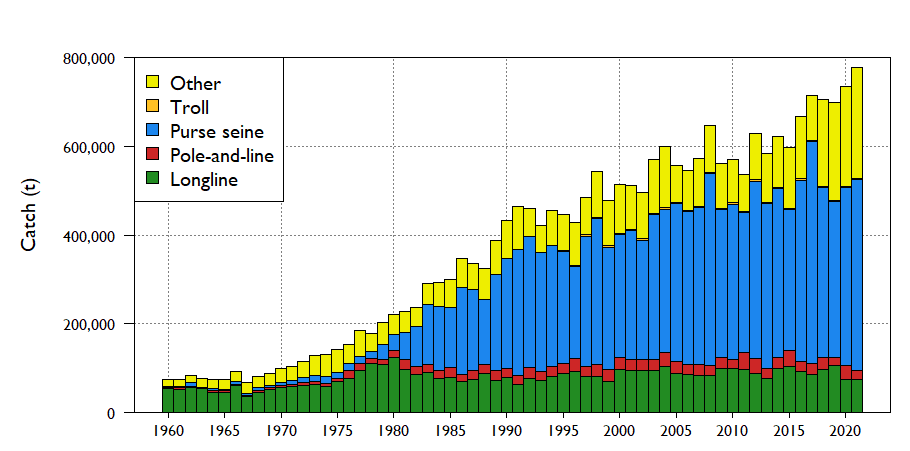
\includegraphics [width=15cm]{Fig10a-yft_catchbygearE.png}
  \caption {Distribution of total .\label{fig3}}
\end{figure}
\clearpage

\hypertarget{bigeye-tuna}{%
\section{Bigeye tuna}\label{bigeye-tuna}}

The most recent bigeye tuna assessment was conducted in 2020
(\textbf{cite}). The bigeye assessment used a nine region model, your
EEZ is situated in \textbf{betreg} (\autoref{fig4} - top). Between
\textbf{minyear} and \textbf{maxyear} bigeye catch averaged
\textbf{tabl2}t in the WCPFC-CA (\autoref{fig4} - middle). An average of
\textbf{tabl2}t (\textbf{tabl2}\% of WCPFC-CA catch) comes from
\textbf{betreg}. It is estimated that bigeye spawning biomass in the
WCPFC-CA and \textbf{betreg}, have declined by \textbf{tabl2}\% and
\textbf{tabl2}\% respectively (\autoref{tab2}). The greatest impact on
spawning biomass is from the associated - FAD - purse seine fisheries in
the WCPO and from the longline fishery in \textbf{betreg}
(\autoref{fig4} - bottom).

The SC14 concluded that overfishing is not occurring on the bigeye stock
and the stock is not overfished (\autoref{fig1}). However, the increase
in juvenile bigeye catch has resulted in a considerable reduction in the
potential yield of the WCPO bigeye stock. The loss in yield per recruit
due to excess harvest of juvenile fish is substantial.

Annual catch of bigeye in the Solomon Islands have averaged
\textbf{tabl2}t between \textbf{minyear} and \textbf{maxyear},
representing \textbf{tabl2}\% of WCPFC-CA and \textbf{tabl2}\% of
\textbf{betreg} bigeye catch. Together, bigeye catch inside the Solomon
Islands and by your fleet outside your EEZ have accounted for an average
\textbf{tabl2}\% of the WCPFC bigeye catch. Regional catch of bigeye
tuna, including those within or by the Solomon Islands, are considered
to be low if maintained at recent average levels. However, the Solomon
Islands should note that the FAD component of the regional purse seine
fishery (the main fishery for skipjack tuna) catches juvenile bigeye and
yellowfin tuna, and that fishery is contributing to the impact on this
stock.

Bigeye tuna is one of two species targeted in the longline fishery
operating in the Solomon Islands* and is also taken in the purse seine
fishery in the Solomon Islands. The viability of the local and regional
purse seine fishery is not dependent on bigeye tuna abundance. However,
the prospects for long-term viability (and/or further expansion) of a
longline fishery for bigeye in the Solomon Islands will be dependant, in
part, on trends in both national and regional fishing mortality on the
bigeye stock (and economic and other factors not discussed here).

\clearpage

\begin{figure}[!ht]
 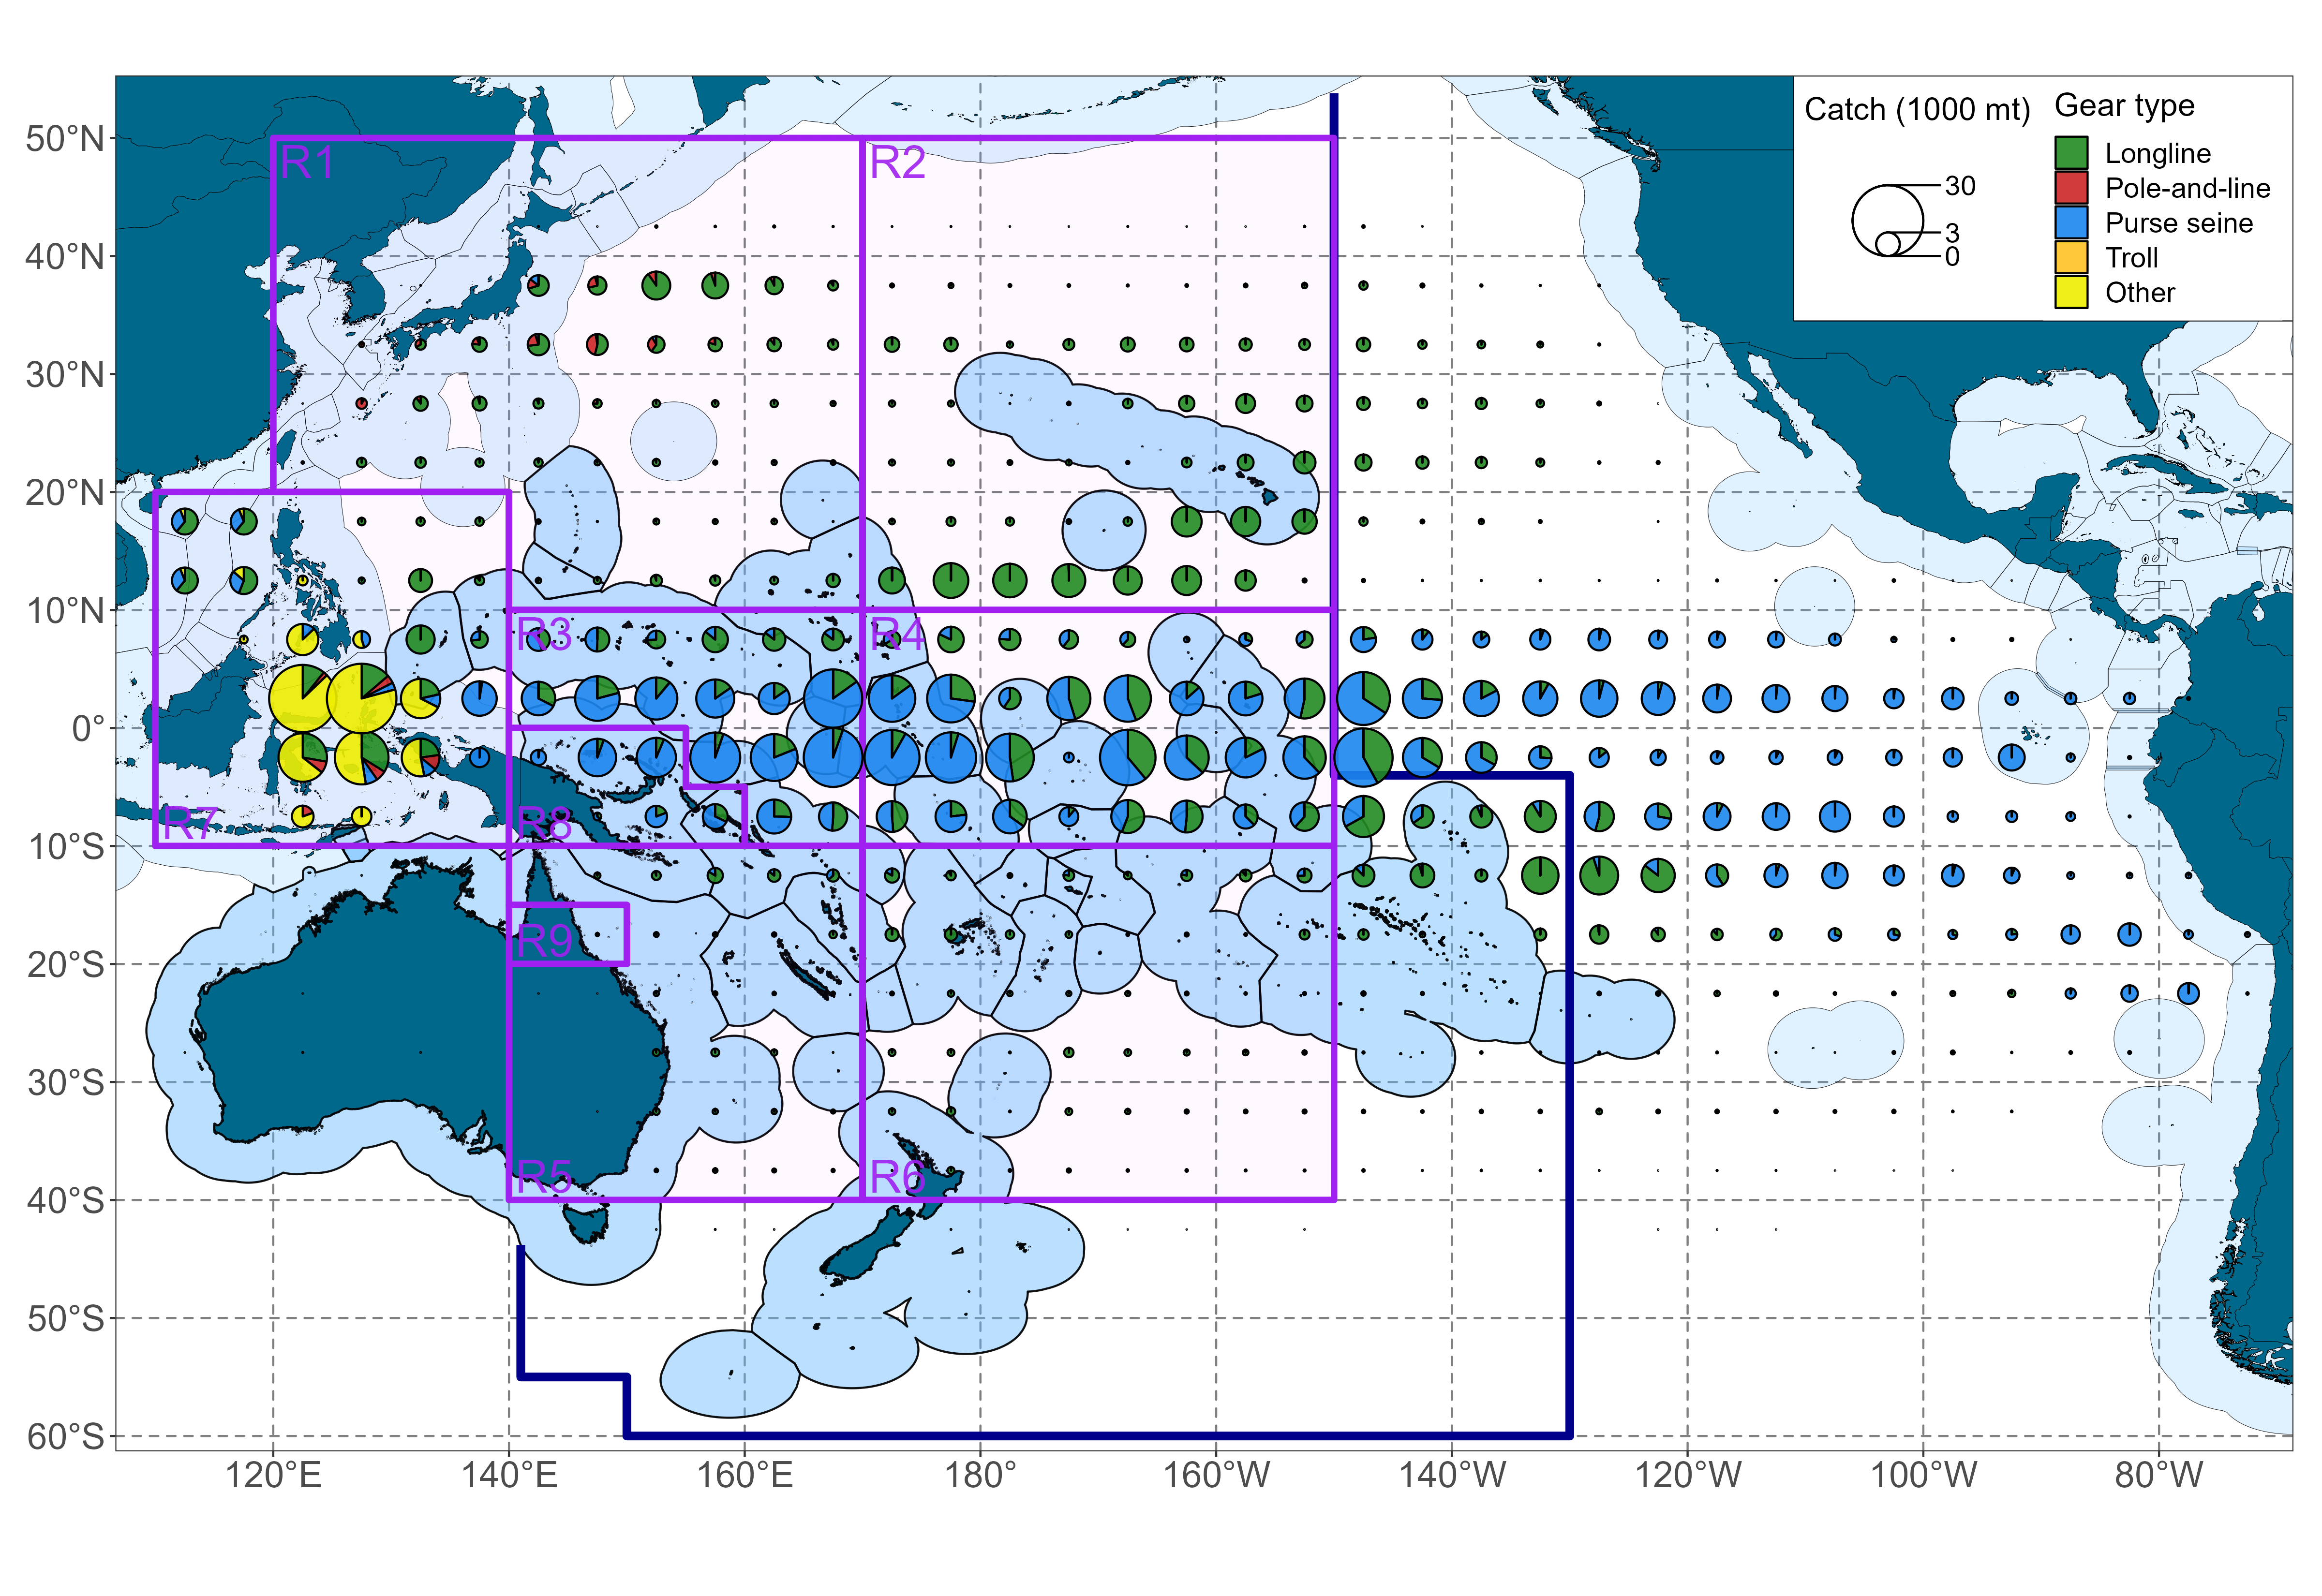
\includegraphics [width=15.5cm]{Fig12b-bet_mapE.png}
 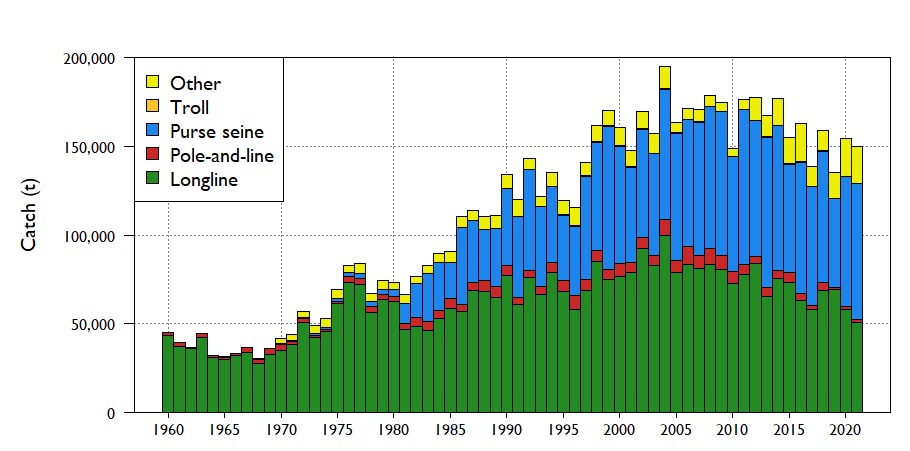
\includegraphics [width=15cm]{Fig12a-bet_catchbygearE.png}
   \caption {Distribution of total .\label{fig4}}
\end{figure}
\clearpage

\hypertarget{south-pacific-albacore-tuna}{%
\section{South Pacific albacore
tuna}\label{south-pacific-albacore-tuna}}

The most recent south Pacific albacore (hereafter, simply ``albacore'')
assessment was conducted in 2021 \textbf{TremblayBoyer2018}. The
albacore assessment used a five region model, your EEZ is situated in
\textbf{albreg} (\autoref{fig5} - top). Between \textbf{minyear} and
\textbf{maxyear} albacore catch averaged \textbf{tabl2}t in the WCPFC-CA
(\autoref{fig5} - middle). An average of \textbf{tabl2}t
(\textbf{tabl2}\% of WCPFC-CA catch) comes from \textbf{albreg}. It is
estimated that albacore spawning biomass in the WCPFC-CA and
\textbf{albreg}, have declined by \textbf{tabl2}\% and \textbf{tabl2}\%
respectively (\autoref{tab2}). The greatest impact on spawning biomass
is from the sub-tropical longline fisheries both in the WCPO and in
\textbf{albreg} (\autoref{fig5} - bottom).

The WCPFC \textbf{SC14} concluded that South Pacific albacore spawning
stock is currently above both the level that will support the MSY and
the adopted spawning biomass limit reference point, and overfishing is
not occurring (\autoref{fig1}). But \textbf{SC14} also noted that while
overfishing is not occurring, further increases in effort will yield
little or no increase in long-term catch and result in further reduced
catch rates. \textbf{SC14} also noted that any increases in catch or
effort in sub-tropical longline fisheries are likely to lead to declines
in longline catch rates between 10\(^o\)S-30\(^o\)S, which will impact
vessel profitability \textbf{WCPFC2018}. An interim Target Reference
Point of \(SB/SB_{F=0}\) = 0.56 was adopted in 2019 \textbf{WCPFC2019};
the current spawning biomass level of 0.52 is estimated to be below the
interim TRP

Annual catch of albacore in the Solomon Islands has averaged
\textbf{tabl2}t between \textbf{minyear} and \textbf{maxyear},
representing \textbf{tabl2}\% of WCPFC-CA and \textbf{tabl2}\% of
\textbf{albreg} albacore catch. Together, albacore catch inside the
Solomon Islands and by the Solomon Islands fleet outside your EEZ have
accounted for an average \textbf{tabl2}\% of the WCPFC albacore catch.
Regional catch of albacore tuna, including those within or by Solomon
Islands vessels fishing outside your EEZ, are considered sustainable at
recent average levels. But ct.long should note that, deterministic
projections\footnote{Estimates of risk using deterministic projections are likely to be underestimated as they do not include future uncertainties such as fluctuations in recruitment.}
\textbf{Pilling2018} estimate that there is a 24\% chance of the overall
stock falling below the LRP by 2045 at recent (status quo) catch and
effort levels. While the stock remains in a biologically healthy state,
the prospects for any future albacore targeted fishery in the Solomon
Islands will depend on local abundance, catch rates and economics.

\clearpage

\begin{figure}[!ht]
 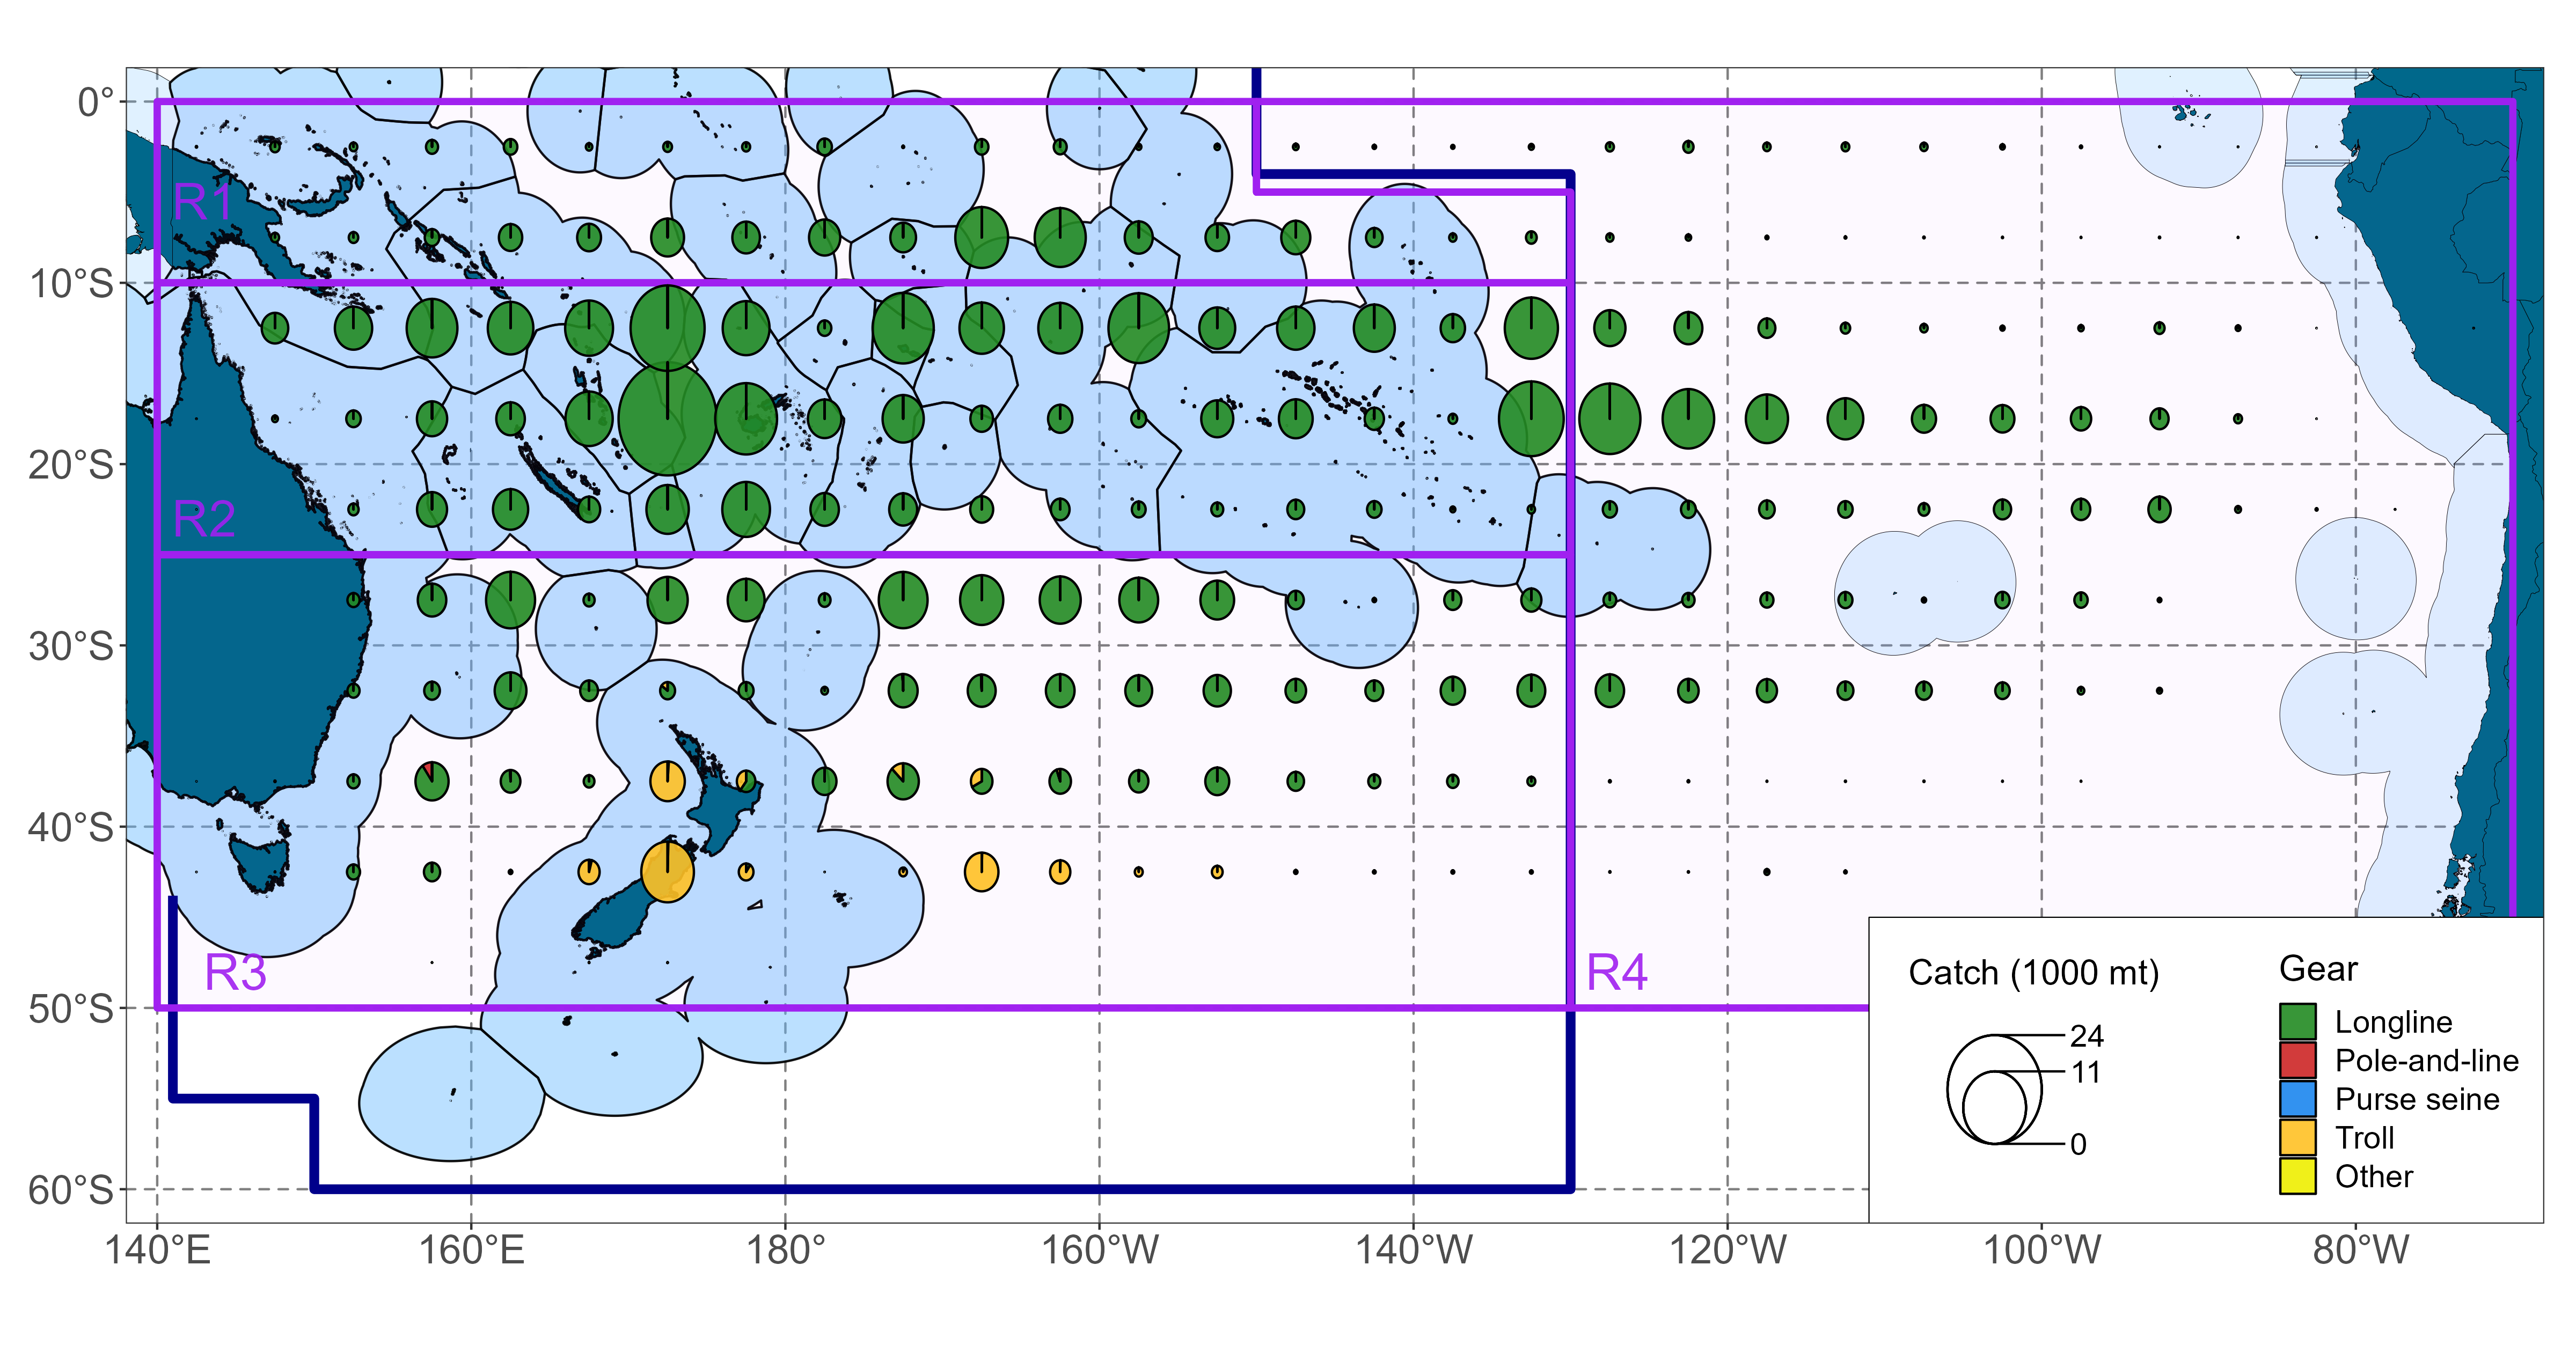
\includegraphics [width=15.5cm]{Fig14b-alb_mapE.png}
 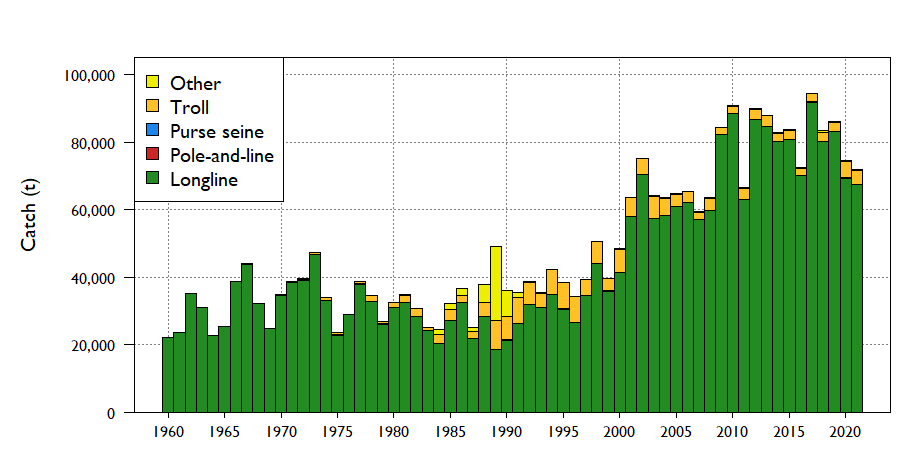
\includegraphics [width=15cm]{Fig14a-alb_catchbygearE.png}
  \caption {Distribution of total South Pacific albacore catch by fishing method 2009-2018 (Red, pole-and-line; Blue, purse-seine; Green, longline; Yellow, other) (top).  Annual catch of South Pacific albacore in the WCPO by fishing method (middle). Percentage impact on spawning biomass due to fishing in the WCPO (bottom - left) and the model Region encompassing your EEZ (bottom - right).\label{fig5}}
\end{figure}
\clearpage

\hypertarget{other-species}{%
\section{Other species}\label{other-species}}

Stock assessments are available for some other species which may
interact with the fisheries in the Solomon Islands (\autoref{tab3}).
These include three shark and three billfish species (\autoref{fig6}).
Both north and south Pacific swordfish and blue marlin are not
overfished and no overfishing was taking place. The SC, has recommended
that there should be no increase in fishing mortality for blue marlin
and swordfish. The southwest Pacific striped marlin assessment results
indicate that the stock is fully exploited, is not experiencing
overfishing, but may be overfished (\autoref{tab3}) \textbf{WCPFC2012}
\textbf{WCPFC2013b}. For the sharks that have been assessed to date,
blue sharks in the north Pacific are not considered to be overfished and
no overfishing is taking place; silky sharks are overfished and
overfishing is taking place; and for oceanic whitetip sharks the stock
is overfished and overfishing is occuring
\textbf{WCPFC2012,WCPFC2013,WCPFC2014}. It should also be noted that due
to concerns expressed by the Scientific Committee regarding the steep
declines in biomass of silky and oceanic whitetip shark, the Commission
has adopted CMMs for these species prohibiting their retention,
transshipment, storage or landing \textbf{WCPFC2011a, WCPFC2013b}. In
addition, in an attempt to reduce incidental catch of these species
CMM2014-05 prohibits the use of either wire trace branchlines or shark
lines on longline sets \textbf{this has now changed?}.

\begin{figure}[!ht]
 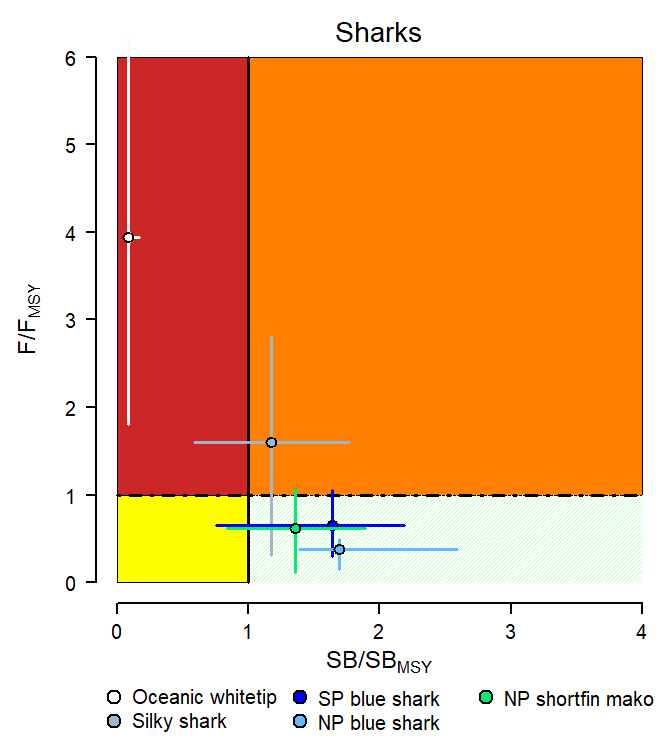
\includegraphics [width=11.5cm]{Fig23b-shark.kobe.crosshairs.png} 
 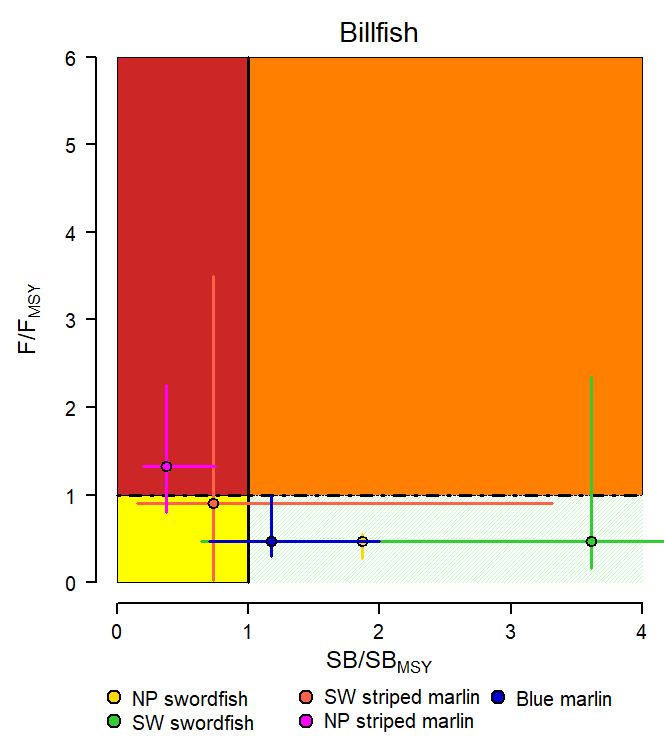
\includegraphics [width=11.5cm]{Fig23a-billfish.kobe.crosshairs.png} 
  \caption {Kobe plots comparing the stock status of the key bycatch species caught in the WCPFC Convention Area. Where current fishing mortality rate exceeds the fishing mortality rate at MSY (F/F$_{MSY}$ > 1) then overfishing is occurring. Where the current spawning biomass is less than the spawning biomass that would produce MSY, then the stock is overfished (SB/SB$_{MSY}$ <1). \label{fig6}}  
\end{figure}
\clearpage

\begin{table}[h]
\fontsize{9pt}{9pt}\selectfont
\begin{tabular}{p{2cm}p{1cm}p{2cm}p{6cm}p{4cm}}
\hline
Species/Stock & Assesed & Status & SC Recommendation & Reference \\ \hline
Blue marlin & 2021 &  No overfishing, not overfished & Need for improved biological data for all billfish species withinthe WCPFC convention areal & (SC19-SA-WP-16, WCPFC20-2023-SC19-01) \\
Striped marlin (SWPO) & 2019 & Stock fully exploited, not experiencing overfishing but is overfished & Need for improved biological data for all billfish species withinthe WCPFC convention areal & (SC19-SA-IP-11, WCPFC20-2023-SC19-01) \\ 
North Pacific Swordfish & 2023 & No overfishing, not overfished & NP SWO stock status is positive with no evidence of excess F above FMSY or substantial depletion of spawning potential & (WCPFC20-2023-SC19-01, SA-WP-16-rev-1) \\
Swordfish (SPO) & 2021 & SWPO stock - No overfishing, not overfished & Develop sex disaggregated models to account for the significant differences in life history between the sexes  and relatively simple single region spatial structure represent key areas of uncertainty in the assessment. & (SA-WP-16-rev-1) \\
Southwest Pacific Blue shark & 2022 & No overfishing, not overfished & Catch and fishing effort on blue shark should be carefully monitored & (SC17-SA-WP03; SC17-SA-IP-06, SC17-SA-IP-19) \\
North Pacific Blue shark (NP) & 2022 & No overfishing, not overfished & Catch and fishing effort on blue shark should be carefully monitored & (SC18-SA-WP-06, SC19-EB-WP-06) \\
Oceanic whitetip shark & 2019 & Overfishing, overfished & Management measures to reduce fishing mortality and to rebuild spawning biomass required and mitigation to avoid capture is recommended. & (SC19-EB-WP-06) \\
Silky shark & 2023 & Overfishing occurring, however not overfished & Develop mitigation as well as measures control targeted catch. & (SC19-EB-WP-06) \\
\hline
\label{tab3}
\end{tabular}
\caption{Stock status and WCPFC Scientific Committee (SC) recommendations for non-key tuna species stocks caught in the WCPFC-CA. NP = North Pacific; SWPO = Southwest Pacific Ocean; SPO = South Pacific Ocean; SEPO=Southeast Pacific Ocean.} 
\end{table}


\hypertarget{references}{%
\section{References}\label{references}}

\hypertarget{refs}{}
\begin{CSLReferences}{1}{0}
\leavevmode\vadjust pre{\hypertarget{ref-Brouwer2019_a}{}}%
Brouwer, S., G. Pilling, P. Williams, and J. Hampton. 2019. {``A
Compendium of Fisheries Indicators for Tuna Stocks.''}
WCPFC-SC15-2019/SA-WP-01. Pohnpei, Federated States of Micronesia, 12 -
20 August 2019.

\leavevmode\vadjust pre{\hypertarget{ref-Vincent2019_a}{}}%
Vincent, M, G P Pilling, and J Hampton. 2019. {``Stock Assessment of
Skipjack Tuna in the Western and Central Pacific Ocean.''}
WCPFC-SC15-2019/SA-WP-05-Rev2. Pohnpei, FSM, 12--20 August 2019.

\end{CSLReferences}

\vspace*{\fill}
\clearpage

\hypertarget{tables}{%
\section*{Tables}\label{tables}}
\addcontentsline{toc}{section}{Tables}

\hypertarget{figures}{%
\section{Figures}\label{figures}}

\end{document}
